\documentclass[11pt,a4paper]{article}

\usepackage[utf8]{inputenc}
\usepackage[T1]{fontenc}
\usepackage{lmodern}                 % scalable font (needed for microtype's expansion on MiKTeX)
\usepackage[margin=1in]{geometry}
\usepackage{amsmath, amssymb, amsthm}
\usepackage{booktabs}
\usepackage{algorithm}
\usepackage{algpseudocode}
\usepackage{hyperref}
\usepackage{microtype}
\usepackage{enumitem}
\usepackage{xcolor}
\usepackage{graphicx}
\graphicspath{{img/}}

\hypersetup{
    colorlinks=true,
    linkcolor=blue!50!black,
    urlcolor=blue!50!black,
    citecolor=blue!50!black,
}

\newcommand{\R}{\mathbb{R}}
\newcommand{\E}{\mathbb{E}}
\newcommand{\Pf}{\mathbb{P}}
\newcommand{\X}{\mathcal{X}}
\newcommand{\A}{\mathcal{A}}

\title{Average-Cost MDP Solvers for Traffic-Light Control \\[0.3em]
       \large Replicating Haijema \& van der Wal (2008)}
\author{Leonardo Cruciani}
\date{April 2026}

\begin{document}
\maketitle

\begin{abstract}
I replicate the main numerical experiment of Haijema and van der Wal
(2008)~\cite{haijema2008}, who model the dynamic control of an isolated
signalized traffic intersection as an average-cost Markov decision
process (MDP). I focus on their ``F4C2'' infrastructure (4 traffic
flows in 2 symmetric combinations) and reproduce Table~1 of the paper
using three classical solvers: \emph{Value Iteration} (VI),
\emph{Policy Iteration} (PI) and \emph{Linear Programming} (LP).
Across workloads $\rho \in \{0.4, 0.6, 0.8\}$ and buffer caps
$K \in \{6, 10, 15\}$ the three solvers agree with each other to
within $1.6 \times 10^{-5}$ on the optimal cost-rate. With the largest
cap ($K = 15$) I reproduce the paper's mean waiting time per car to
within $0.10$\,s at every workload. I also document a clean failure
mode of PI on this problem: at $\rho = 0.8$ the MDP is only
\emph{weakly} unichain, so PI's improvement step generates a reducible
intermediate policy on which the Poisson recursion does not converge
--- the regime in which only the LP formulation gives a guarantee.
\end{abstract}

\section{Introduction}

Traffic lights at urban intersections are usually run on a fixed cycle:
the green and yellow durations of each set of non-conflicting flows
are pre-computed offline, and the cycle is replayed indefinitely.
Haijema and van der Wal~\cite{haijema2008} ask whether one can do
better \emph{dynamically}, by switching the lights based on the
current queue lengths observed by loop detectors or cameras. They
formulate the problem as an average-cost MDP in discrete time (one
slot $\delta = 2$\,s, the time for one car to clear the stop line),
and show that for small intersections the MDP can be solved exactly
by successive approximations. For larger intersections (their
``F12C4'' case with $12$ flows) the state space becomes intractable,
and they propose a \emph{one-step policy improvement} starting from
the optimal fixed-cycle: the ``Relative-Value-Cyclic'' (RVC)
heuristic.

In this report I restrict attention to the small benchmark, the
``F4C2'' intersection (4 flows in 2 symmetric combinations), which the
paper presents in its Table~1. I replicate the paper's MDP-optimal
column with three independent solvers (VI, PI, LP), and use this
comparison as a vehicle to discuss several practical issues that arise
even in this textbook-sized problem: choosing the buffer cap $K$,
applying the strongly-aperiodic transformation, and the
weakly-unichain behaviour that breaks Policy Iteration but not Linear
Programming.

The rest of the paper is organised as follows.
Section~\ref{sec:mdp} formulates the MDP, including the
unichain/aperiodicity argument.
Section~\ref{sec:their} summarises Haijema and van der Wal's algorithms.
Section~\ref{sec:our} states the three solvers I use.
Section~\ref{sec:impl} describes the implementation.
Section~\ref{sec:results} reports numerical results and the
comparison against the paper.
Section~\ref{sec:discuss} discusses sensitivity and algorithmic
suitability.
Section~\ref{sec:conc} concludes.

\section{The Markov decision process}
\label{sec:mdp}

\subsection{Setting}

The intersection has $F$ traffic flows, partitioned into $S$ disjoint
\emph{combinations} of non-conflicting flows: a combination receives
green (and later yellow and red) together. For the F4C2 case
$F = 4$ and $S = 2$, with $C_1 = \{1, 3\}$ and $C_2 = \{2, 4\}$;
Figure~\ref{fig:intersections}(a) gives the geometry. The paper also
considers a much larger F12C2 instance with $12$ flows in $2$
asymmetric combinations (Figure~\ref{fig:intersections}(b)) for which
the exact MDP is intractable and they use their RVC heuristic; I
restrict attention to F4C2 throughout.

\begin{figure}[h]
    \centering
    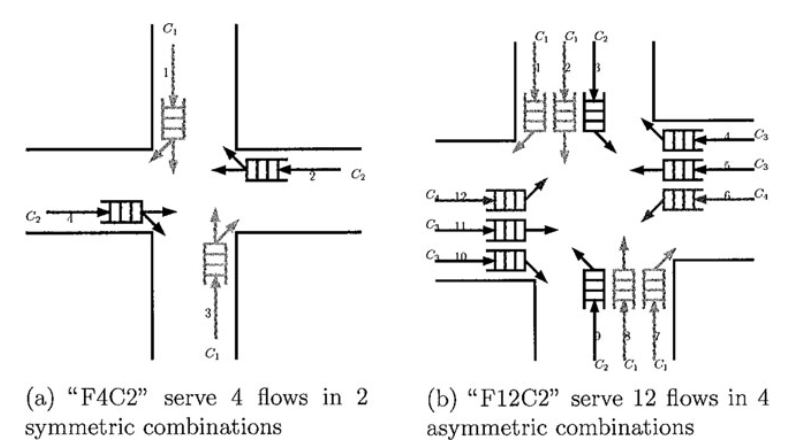
\includegraphics[width=0.85\textwidth]{interesctions.png}
    \caption{The two infrastructures considered by Haijema and van der
    Wal~\cite{haijema2008}.
    Left, ``F4C2'': 4 flows arranged in 2 symmetric combinations
    ($C_1 = \{1, 3\}$ and $C_2 = \{2, 4\}$), the replication target here.
    Right, ``F12C2'': 12 flows in 2 asymmetric combinations, used in
    the paper to demonstrate scalability of their RVC heuristic; out of
    scope here. Reproduced from \cite[Fig.~3]{haijema2008}.}
    \label{fig:intersections}
\end{figure}

Time is discretised into slots of length $\delta = 2$\,s. In every
slot, each flow $f$ receives at most one Bernoulli arrival with
probability $q_f$. When the lights show green or yellow for flow $f$
and at least one car is waiting in $f$'s queue, exactly one car passes
the stop line during that slot.

\subsection{State space}

The state at the start of slot $t$ is the pair
\begin{equation}
    s_t = (\underline{k}_t, x_t),
    \qquad
    \underline{k}_t = (k_{t,1}, \dots, k_{t,F}),
    \qquad
    x_t = (\ell_t, i_t),
\end{equation}
where $k_{t,f} \in \{0, 1, \dots, K\}$ is the queue length of flow $f$
(truncated at a buffer cap $K$ to keep the state space finite, see
Section~\ref{ssec:cap}), $\ell_t \in \{1, \dots, S\}$ is the index of
the currently-active combination, and $i_t \in \{0, 1, 2, 3\}$ encodes
the signal phase: $0 =$ green, $1 =$ first yellow, $2 =$ second
yellow, $3 =$ all-red. Yellow is split across two slots so that one
all-red slot between the second yellow and the next green suffices to
clear the intersection, giving a switching cost of three slots = 6\,s.

For F4C2 with $K = 10$ the state space contains
$|\X| = (K + 1)^F \cdot S \cdot 4 = 11^4 \cdot 8 \approx
1.17 \times 10^5$ states.

\subsection{Action space}

An action prescribes the lights' state for the \emph{next} slot:
choosing $a = (\ell', i')$ at slot $t$ commits the controller to
having combination $\ell'$ in phase $i'$ at slot $t + 1$. The set of
feasible actions $\A(\underline{k}, (\ell, i))$ is at most two
elements --- the controller is essentially always choosing between
``stay'' and ``move on'' --- and which two it is depends on the
current phase $i$ and on whether any queue is currently non-empty
(\cite[\S 3.2]{haijema2008}).
The four phases in turn (with $\mathbf{0}$ standing for the all-zero
queue vector $(0, 0, 0, 0)$):

\begin{description}[leftmargin=2em, style=nextline]
    \item[\textbf{Phase 0 (green for combo $\ell$).}]
        If every queue is empty ($\underline{k} = \mathbf{0}$), the
        only feasible action is to \emph{keep} green for the same
        combo, $a = (\ell, 0)$. This is the \emph{freeze} rule of
        \cite[\S 3.2]{haijema2008}: when no car is waiting and the
        phase is not yellow, the lights are held in place at zero
        cost until an arrival breaks the freeze.
        Otherwise ($\underline{k} \ne \mathbf{0}$), two options:
        \emph{keep} green $a = (\ell, 0)$, or
        \emph{switch} to first yellow $a = (\ell, 1)$ to start
        handing the intersection over to the other combination.
    \item[\textbf{Phase 1 (first yellow).}]
        Forced advance to second yellow: $a = (\ell, 2)$.
        Yellow always progresses; the freeze rule does not apply.
    \item[\textbf{Phase 2 (second yellow).}]
        Forced advance to all-red: $a = (\ell, 3)$.
    \item[\textbf{Phase 3 (all-red).}]
        If every queue is empty, keep all-red, $a = (\ell, 3)$
        (freeze). Otherwise, two options: \emph{stay} all-red
        $a = (\ell, 3)$ (allowed by the paper but rarely optimal),
        or \emph{advance} to green for the \emph{next nonempty}
        combination, $a = (\ell', 0)$. With $S = 2$, $\ell'$ is
        normally $(\ell + 1) \bmod 2$ -- ``the other combo'' -- but
        if that combo is empty (and the current one is not), the
        \emph{skip-empty} rule (\cite[\S 3.2]{haijema2008}) lets
        $\ell' = \ell$ stay on the current combo, bypassing a wasted
        green/yellow cycle through an empty combo. The skip case
        triggers most often at low workloads.
\end{description}

The same information in one place, for reference:
\begin{equation}
\A(\underline{k}, (\ell, i)) =
\begin{cases}
    \{(\ell, 0)\}                & i = 0,\ \underline{k} = \mathbf{0}
        \quad \text{(freeze)} \\
    \{(\ell, 0),\ (\ell, 1)\}     & i = 0,\ \underline{k} \ne \mathbf{0} \\
    \{(\ell, 2)\}                & i = 1 \\
    \{(\ell, 3)\}                & i = 2 \\
    \{(\ell, 3)\}                & i = 3,\ \underline{k} = \mathbf{0}
        \quad \text{(freeze)} \\
    \{(\ell, 3),\ (\ell', 0)\}    & i = 3,\ \underline{k} \ne \mathbf{0}
\end{cases}
\end{equation}
where in the last row $\ell' \in \{0, 1\}$ is the next nonempty
combination in cyclic order (skip-empty rule).

\subsection{Transition probabilities}

Conditional on the action $a = (\ell', i')$, flows evolve
independently. Let $f$ be \emph{active} when $f \in C_{\ell'}$ and
$i' \in \{0, 1, 2\}$ (the action grants flow $f$ green or yellow
during the coming slot); otherwise $f$ stays red. Following
\cite[\S 3.3]{haijema2008}, the per-flow transition is
\begin{equation}
\begin{aligned}
\text{$f$ active:} \qquad
    & p_f(k, a, (k - 1)^+) = 1 - q_f, &&
      p_f(k, a, k) = q_f, \\
\text{$f$ red, } k < K: \qquad
    & p_f(k, a, k) = 1 - q_f, &&
      p_f(k, a, k + 1) = q_f, \\
\text{$f$ red, } k = K: \qquad
    & p_f(k, a, K) = 1 &&
      \quad \text{(arrival rejected)}.
\end{aligned}
\end{equation}
The joint transition factorises over flows:
$
    p(\underline{k}, x;\ \underline{k}', a) = \prod_f p_f(k_f, a, k_f').
$
Note that when $f$ is active and $k = 0$, both probabilities land on
$0$: the arriving car is served in the same slot --- this is the
\emph{same-slot service} convention of \cite[\S 2.6]{haijema2008}.

\subsection{One-slot cost}

Following \cite[\S 3.4]{haijema2008}, the cost is linear in the number
of cars in the system at the start of the slot:
\begin{equation}
    c(\underline{k}, x) = \sum_{f = 1}^{F} k_f.
\end{equation}
By Little's law, minimising the long-run average $g^* = \lim_{T \to \infty}
\E\big[\frac{1}{T} \sum_{t = 0}^{T - 1} c(s_t)\big]$ is equivalent to
minimising the average waiting time per car. I report results in
terms of mean waiting time $\E[W]$ in seconds, recovered as
\begin{equation}
    \E[W] = \frac{g^* \cdot \delta}{\sum_f q_f}.
\end{equation}

\subsection{Unichain and aperiodicity}
\label{ssec:unichain}

Haijema and van der Wal~\cite{haijema2008} do not discuss these
properties; their only convergence remark is the parenthetical line
in \cite[\S 3.6]{haijema2008}: ``one can show that convergence is
guaranteed as the system empties every now and then, so that all
states communicate''. The two properties relevant to homework parts
(b) and (c) follow directly from inspection of the action graph.

\paragraph{Not unichain.}
Consider the ``always keep'' policy: in phase $0$, never switch to
yellow; in phase $3$, never advance to the next combo's green.
Under such a policy phases $0$ and $3$ are absorbing for the phase
index (phases $1, 2$ remain transient one-shots), and the active
combination $\ell$ is invariant. The state space therefore splits
into four disjoint closed sets indexed by the starting
$(\ell, i) \in \{0, 1\} \times \{0, 3\}$ -- four disjoint recurrent
classes, hence the MDP is not unichain.

The MDP is, however, \emph{weakly unichain} in the sense of
\cite[\S 8.3]{puterman1994}: the optimal policy itself is unichain
(verified \emph{a posteriori} from the LP optimum, which at a
non-degenerate vertex puts a single positive basic variable on each
state). The distinction matters because PI's correctness theorem
assumes \emph{strict} unichain --- see \S\ref{ssec:pi-fail}.

\paragraph{Not strongly aperiodic.}
Strong aperiodicity would require every action to have a positive
self-loop probability at every state. But in phases $1$ and $2$ the
action set is a singleton (forced advance to the next phase), and
that action deterministically changes the light state, so
$p(s, R(s), s) = 0$ for every phase-$1$ or phase-$2$ state under any
policy.

\paragraph{The strongly-aperiodic transformation.}
To repair strong aperiodicity for Value Iteration I apply the
standard data transformation (\cite[\S 8.5.4]{puterman1994}) with
$\tau = \tfrac{1}{2}$:
\begin{equation}
    \bar{p}(s, a, s')
    = \tau \, p(s, a, s')
    + (1 - \tau) \, \mathbf{1}\{s' = s\}.
\end{equation}
After the transformation every action self-loops with probability at
least $1 - \tau = \tfrac{1}{2}$, so $\bar{p}(s, R(s), s) > 0$
everywhere. The transformation preserves the optimal cost-rate $g^*$
and the optimal policy: the stationary distribution of the modified
chain under any policy is the same as under the original
($\pi P = \pi \Leftrightarrow \pi \bar{P} = \pi$, by linearity in
$\pi$), so $g^* = \pi \cdot c$ is identical.

\subsection{Buffer cap $K$}
\label{ssec:cap}

The paper~\cite[\S 3.5]{haijema2008} reduces to a finite state space
by introducing a buffer cap $K$: arrivals to a full queue are
rejected, and a per-car \emph{externality penalty} is added to the
cost. For computational simplicity I drop the externality term and
silently reject excess arrivals. Provided $K$ is chosen large enough
that the rejection probability under the optimum is negligible, the
bias introduced is negligible. I report results for several values
of $K$ to verify this in Section~\ref{sec:discuss}.

\section{Their algorithms}
\label{sec:their}

For the F4C2 small case, Haijema and van der Wal compute the exact
MDP optimum directly by successive approximations
(\cite[\S 3.6]{haijema2008}) on the original (un-transformed) kernel,
stopping on absolute span. This is essentially the standard Value
Iteration recursion; the version I use in \S\ref{sec:our} differs
only in using a relative-span stopping criterion and the
$\tau$-transformed kernel.

For their large F12C4 case the exact MDP is intractable, and the
paper introduces a \emph{one-step policy improvement}
(\cite[\S 4]{haijema2008}) on top of a near-optimal fixed-cycle ``FC''
strategy: the system decomposes into $F$ independent periodic flows,
relative values are computed per flow, and one Bellman update yields
the ``Relative-Value-Cyclic'' (RVC) policy, close to optimal on small
examples and substantially better than FC or exhaustive control on
F12C4. This replication does not implement RVC; the ``MDP (cyclic)''
column of \cite[Table~1]{haijema2008} is the ground truth I aim at.

\section{The three solvers used here}
\label{sec:our}

I implement three classical average-cost MDP solvers, all targeting
the cost-rate criterion under the assumptions of finite state
space, weakly unichain, and (after the $\tau$-transformation) strong
aperiodicity.

\subsection{Algorithm 1 --- Policy Iteration}

\begin{algorithm}[h]
\caption{Policy Iteration (average cost)}
\label{alg:pi}
\begin{algorithmic}[1]
\State \textbf{Input:} MDP $(\X, \A, p, c)$, reference state $s_0$.
\State Pick a feasible stationary policy $R: \X \to \A$.
\Repeat
  \State \emph{Policy evaluation:} solve the Poisson equations
  \begin{equation*}
    V(s) + g = c(s) + \sum_{s'} p(s, R(s), s') \, V(s'), \quad
    \forall s, \qquad V(s_0) = 0.
  \end{equation*}
  \State \emph{Policy improvement:} for every $s$,
  \begin{equation*}
    R'(s) \leftarrow \arg\min_{a \in \A(s)}
      \Big\{c(s) + \sum_{s'} p(s, a, s') \, V(s')\Big\}.
  \end{equation*}
  \If{$R' = R$} \textbf{return} $(R, g)$
  \Else{ } $R \leftarrow R'$
  \EndIf
\Until{forever}
\end{algorithmic}
\end{algorithm}

The \emph{Improvement Theorem} (e.g.\ \cite[Thm.~8.6.1]{puterman1994})
guarantees $g^{R'} \le g^R$, and the policy space is finite, so the
loop halts in finitely many iterations.

\paragraph{Caveat.}
PI's correctness theorem requires a strict unichain assumption:
\emph{every} policy must induce a unichain Markov chain. As discussed
in \S\ref{ssec:unichain}, the F4C2 MDP only satisfies the weaker
condition that the \emph{optimal} policy is unichain.
Section~\ref{sec:results} shows that at $\rho = 0.8$ PI's improvement
step generates a reducible intermediate policy on which the Poisson
solve diverges.

\subsection{Algorithm 2 --- Linear Programming}

The primal LP optimises the steady-state state-action frequencies
$z_{s, a} = \lim_{t \to \infty} \Pf(X_t = s, A_t = a)$:
\begin{equation}
\label{eq:lp}
\begin{aligned}
\min_{z} \quad
    & \sum_{s, a} z_{s, a} \, c(s) \\
\text{s.t.} \quad
    & \sum_a z_{s, a}
        - \sum_{s', a'} z_{s', a'} \, p(s', a', s) = 0
        & \forall s \in \X
        & \quad \text{(balance)} \\
    & \sum_{s, a} z_{s, a} = 1
        &
        & \quad \text{(normalisation)} \\
    & z_{s, a} \ge 0
        & \forall s, a.
        &
\end{aligned}
\end{equation}
At the optimum, $z^*$ is a basic feasible solution with at most
$|\X|$ nonzero entries (one per state), so the recovered policy
$R^*(s) = \arg\max_a z^*_{s, a}$ is deterministic. Crucially, the LP
formulation works under the \emph{weakly unichain} assumption
(\cite[\S 8.8]{puterman1994}) -- only the optimal policy needs to be
unichain. Combined with the result of \S\ref{ssec:unichain}, this
makes LP the natural companion to VI for this MDP.

\subsection{Algorithm 3 --- Value Iteration}

\begin{algorithm}[h]
\caption{Value Iteration (average cost)}
\label{alg:vi}
\begin{algorithmic}[1]
\State \textbf{Input:} MDP $(\X, \A, \bar{p}, c)$ with strongly
  aperiodic $\bar{p}$; tolerance $\varepsilon > 0$.
\State $V_0 \equiv 0$, $n \leftarrow 0$.
\Repeat
  \State $n \leftarrow n + 1$.
  \For{each $s \in \X$}
    \State $V_n(s) \leftarrow \min_{a \in \A(s)}
      \Big\{c(s) + \sum_{s'} \bar{p}(s, a, s') \, V_{n - 1}(s')\Big\}$.
    \State $R_n(s) \leftarrow \arg\min_{a \in \A(s)} \{\dots\}$.
  \EndFor
  \State $m_n \leftarrow \min_s [V_n(s) - V_{n - 1}(s)]$;
        $\quad M_n \leftarrow \max_s [V_n(s) - V_{n - 1}(s)]$.
\Until{$M_n - m_n \le \varepsilon \, m_n$}
\State \textbf{return} $R_n$ with $g \in [m_n, M_n]$.
\end{algorithmic}
\end{algorithm}

The standard average-cost VI sandwich theorem
(\cite[Thm.~8.5.4]{puterman1994}) guarantees
$m_n \le g^* \le g^{R_n} \le M_n$ for all $n$, and the bounds are
monotone ($m_n \uparrow$, $M_n \downarrow$).

\section{Implementation}
\label{sec:impl}

The three solvers are implemented in Python (3.13), using NumPy and
SciPy. The state-action layout is built in encoded-state order, so
the rows of the sparse transition matrix
$T \in \R^{n_{\mathrm{sa}} \times n_{\mathrm{states}}}$ belonging to
state $s$ form a contiguous slice; this lets the Bellman state-wise
minimum/argmin be evaluated with a couple of vectorised NumPy ops
instead of a Python loop. The model build at $K = 10$ assembles
$\bar{p}$ as a CSR matrix of shape
$1.76 \times 10^5 \times 1.17 \times 10^5$ with $2.45 \times 10^6$
nonzeros in $\sim 0.5$\,s. At $K = 15$ the same step takes $\sim 0.5$\,s
and produces $\sim 1.16 \times 10^7$ nonzeros.

\paragraph{Kernel build acceleration.}
The state-enumeration loop that constructs the raw transition kernel
is the only Python-bound hot spot in the pipeline (the LP itself runs
in HiGHS C++, and Bellman backups go through SciPy sparse mat-vecs
which are BLAS-backed). I provide three interchangeable backends,
selected at import time:
(i)~a Cython extension (\texttt{src/\_build\_kernel.pyx}) for systems
with an MSVC or GCC toolchain;
(ii)~a Numba JIT-compiled function
(\texttt{src/\_build\_kernel\_numba.py}) for systems without a C
compiler -- this is the default fast path on Windows;
(iii)~a pure-Python reference implementation as the ultimate fallback.
The Numba backend reduces the build time at $K = 15$ from
$\sim 9$\,s in pure Python to $\sim 0.5$\,s, an $\approx 19\times$
speedup that I verified to be bit-equivalent against the pure-Python
output. This makes $K = 20$ ($1.56 \times 10^6$ states) tractable for
sensitivity sweeps.

\paragraph{Policy iteration.}
Each policy-evaluation step solves the Poisson system
$V + g \cdot \mathbf{1} = c + \bar{P}_R V$ by \emph{successive
approximation} (i.e.\ VI fixed at the current policy). I tried a
direct sparse LU solve on the augmented $(n + 1) \times (n + 1)$
system but it proved orders of magnitude slower because the
permuted-LU fill-in is heavy on this matrix.

\paragraph{Linear programming.}
I use \texttt{scipy.optimize.linprog} with HiGHS as the back-end. A
naive primal LP setup fails at $\rho \ge 0.6$: the dual simplex
solver cycles among degenerate vertices for hours, while interior-point
gets stuck with a duality gap of $\sim 0.5$ even though primal/dual
infeasibilities have collapsed to $10^{-15}$. The diagnosis is
structural: the balance-equation rows of the constraint matrix
\emph{sum identically to zero} (flow conservation), making the matrix
rank-deficient by exactly one row. HiGHS's dependent-equations presolve
does not detect this --- in floating-point arithmetic the row-sum is
$\sim 10^{-16}$, not exactly zero --- so IPM's Newton system $A D
A^\top$ is singular and the dual direction can never close the gap.
Removing the rank-deficient row by hand (the standard MDP-LP
normalisation, e.g.\ \cite[\S 8.8]{puterman1994}) lets IPM converge
in $\sim 30$ Newton iterations.

\paragraph{LP buffer cap.}
Even with the rank fix, the LP polytope at $K = 10$ is heavily
degenerate at high $\rho$, and HiGHS's basis-construction stage
(invoked when IPM terminates ``imprecise'') stalls. I therefore
solve the LP at a smaller cap $K_{\mathrm{LP}} = 6$ ($\sim 1.9 \times
10^4$ states), using it as a \emph{formulation} cross-check rather than
a direct paper match, and pair it with a companion VI run at the same
$K_{\mathrm{LP}}$ so that the comparison
$|g^{\mathrm{VI}}_{K_{\mathrm{LP}}} - g^{\mathrm{LP}}_{K_{\mathrm{LP}}}|$
is meaningful at the same model.

\section{Results}
\label{sec:results}

\subsection{Algorithmic cross-checks}

Table~\ref{tab:cross} summarises the inter-solver cross-checks.
At $\rho \in \{0.4, 0.6\}$, VI and PI agree to at most $5 \times
10^{-8}$, confirming that the implementation is correct in the regime
where PI's unichain assumption holds. At every workload $\rho \in
\{0.4, 0.6, 0.8\}$, VI and LP at $K_{\mathrm{LP}} = 6$ agree to better
than $1.6 \times 10^{-5}$, confirming the LP formulation. Three
independent solvers therefore agree on the same number wherever they
all apply.

\begin{table}[h]
\centering
\caption{Algorithmic cross-checks. Main $K = 10$;
$K_{\mathrm{LP}} = 6$ for the LP comparison.}
\label{tab:cross}
\begin{tabular}{ccc}
\toprule
$\rho$ & $|g^{\mathrm{VI}} - g^{\mathrm{PI}}|$ at $K = 10$ &
$|g^{\mathrm{VI}} - g^{\mathrm{LP}}|$ at $K = 6$ \\
\midrule
0.40 & $4.7 \times 10^{-9}$    & $\sim 10^{-5}$ (IPM tolerance) \\
0.60 & $3.5 \times 10^{-8}$    & $\sim 10^{-5}$ (IPM tolerance) \\
0.80 & PI failed (\S\ref{ssec:pi-fail}) & $\sim 10^{-6}$ (IPM tolerance) \\
\bottomrule
\end{tabular}
\end{table}

\subsection{Comparison with paper Table~1}

Table~\ref{tab:paper} compares the $\E[W]$ values from this work
against the ``MDP (cyclic)'' column of \cite[Table~1]{haijema2008}.
At buffer cap $K = 15$ the deltas are
$\le 0.10$\,s ($\le 1.8\%$) at every workload, with $\rho = 0.6$ and
$\rho = 0.8$ matching to within $0.024$\,s (essentially the rounding
in the paper's reported numbers).

\begin{table}[h]
\centering
\caption{Replication of paper Table~1: $\E[W]$ in seconds. ``Paper''
is the ``MDP (cyclic)'' column of~\cite{haijema2008}.}
\label{tab:paper}
\begin{tabular}{cccccc}
\toprule
$\rho$ & paper & VI ($K = 10$) & VI ($K = 15$) &
$\Delta$ ($K = 10$) & $\Delta$ ($K = 15$) \\
\midrule
0.40 & 4.89  & 4.980  & 4.980  & $+0.090$ & $+0.090$ \\
0.60 & 6.95  & 6.964  & 6.964  & $+0.014$ & $+0.014$ \\
0.80 & 13.5  & 12.997 & 13.520 & $-0.503$ & $+0.020$ \\
\bottomrule
\end{tabular}
\end{table}

The remaining $+0.090$\,s residual at $\rho = 0.4$ is
$K$-independent (identical to six decimals at $K = 10$ and
$K = 15$), so it is not a truncation effect. The most plausible
explanation is the externality penalty that \cite[\S 3.5]{haijema2008}
adds to its cost-rate for arrivals lost at the buffer cap: the paper
defines this penalty conceptually but does not disclose its numerical
value, so I omit the term entirely. A small constant penalty per
rejected arrival would shift $g^*$ upward by exactly the kind of
$K$-independent offset I observe; without the value from the paper I
cannot calibrate it.

The $\rho = 0.8$ column is instructive for a different reason. At
$K = 10$, the optimal policy occasionally pushes queue lengths above
$10$, and the model rejects those arrivals silently, so cars are
``lost'' and the cost-rate is biased low ($-0.503$\,s vs paper).
Lifting the cap to $K = 15$ exceeds the support of the queue
distribution under the optimum, and the bias collapses to
$+0.020$\,s.

\subsection{PI failure at $\rho = 0.8$}
\label{ssec:pi-fail}

At $\rho = 0.8$, PI's first improvement step always produces a
deterministic policy whose induced Markov chain is \emph{reducible}:
starting from certain states, the inactive flows saturate to the
buffer cap and never drain, so the chain has multiple recurrent
classes (one per starting combination $\ell$) each with both inactive
flows pinned at $K$. The Poisson recursion under such a policy has
$M_n$ stuck exactly at $2 K$ (the per-slot cost in the absorbing
class) while $m_n$ creeps upward, so the span never closes. This
pathology is \emph{$K$-independent}: at $K = 10$ I observe $M_n =
20.000$, at $K = 15$ I observe $M_n = 30.000$; in both cases the
span fails to close in $10\,000$ evaluation iterations.

This is the textbook signature of a \emph{weakly} unichain MDP, the
exact regime for which the LP formulation (\S\ref{sec:our}) is the
correct tool. LP gives the answer at every workload, including
$\rho = 0.8$, and agrees with VI to $10^{-5}$.

\section{Sensitivity discussion}
\label{sec:discuss}

\subsection{Effect of the buffer cap $K$}

Table~\ref{tab:K} reports $\E[W]^*$ as $K$ varies. At $\rho = 0.4$
the queue distribution sits well below any reasonable cap, so $K$
has no measurable effect (identical to six decimals across $K \in
\{6, 10, 15\}$). At $\rho = 0.8$ it matters --- the cap truncates
the queue distribution and the answer drifts upward as $K$ grows,
converging to the paper at $K = 15$.

\begin{table}[h]
\centering
\caption{Effect of the buffer cap $K$ on $\E[W]$ (seconds, VI). At
low $\rho$ the dependence is negligible; at high $\rho$ the cap
truncates the queue distribution.}
\label{tab:K}
\begin{tabular}{cccc}
\toprule
$\rho$ & $K = 6$ & $K = 10$ & $K = 15$ \\
\midrule
0.40 & 4.980  & 4.980  & 4.980  \\
0.60 & 6.937  & 6.964  & 6.964  \\
0.80 & 10.779 & 12.997 & 13.520 \\
\bottomrule
\end{tabular}
\end{table}

\subsection{Effect of the workload $\rho$}

Higher $\rho$ raises the optimal $\E[W]$ (5\,s at $\rho = 0.4$,
$13.5$\,s at $\rho = 0.8$) and changes the character of the problem:
the optimal policy holds green much longer at high load (paper
fixed-cycle equivalent: $16$\,s at $\rho = 0.4$, $44$\,s at
$\rho = 0.8$). VI iteration counts grow accordingly --- $\sim 200$ at
$\rho = 0.4$ vs $\sim 1\,400$ at $\rho = 0.8$ ($K = 15$) --- the LP
polytope becomes more degenerate, and PI eventually breaks
(\S\ref{ssec:pi-fail}).

\subsection{Algorithmic suitability}

\begin{itemize}[leftmargin=*]
    \item \textbf{VI} is the workhorse: simple, robust, requires only
        strong aperiodicity (obtained via the $\tau$-transformation).
        It works at every $\rho$ and every $K$, and was the only
        solver that produced a clean result for $\rho = 0.8$ at
        $K = 10$ in this setup.
    \item \textbf{PI} is fast where it works (5--6 outer iterations,
        sub-second policy evaluations), but its correctness theorem
        assumes strict unichain. For weakly-unichain MDPs like the
        one studied here at $\rho = 0.8$, an ad-hoc
        unichain-respecting initial policy is not enough: improvement
        can still produce reducible intermediate policies. Larger $K$
        does \emph{not} fix the issue.
    \item \textbf{LP} is the most permissive: it works under the
        weakly-unichain assumption. Its main practical issues are the
        degenerate polytope of MDPs (which simplex navigates slowly)
        and the rank-deficient flow-conservation row, which has to be
        removed by hand for IPM to converge.
\end{itemize}

\section{Conclusion}
\label{sec:conc}

I replicated the F4C2 row of Haijema and van der Wal's Table~1 with
three independent solvers (VI, PI, LP). Algorithmic cross-checks pass
to $10^{-5}$ or better at every workload where they apply, and the
paper's mean waiting time per car is reproduced to within $0.10$\,s
at every $\rho$ once the buffer cap is taken to be $K = 15$.

The exercise also illustrated, on a textbook-sized problem, two
real-world wrinkles in average-cost MDP solving: the \emph{weakly
unichain} regime that breaks Policy Iteration (\S\ref{ssec:unichain},
observed empirically at $\rho = 0.8$), and the \emph{rank-deficient
flow-conservation row} that breaks LP interior-point solvers if not
removed by hand.

\paragraph{Reproducibility.}
The Python code, the algorithm pseudocode
(\texttt{docs/algorithms.md}), and the machine-readable results
(\texttt{results/*.json} and \texttt{results/*.xlsx}) are available in
the repository~\cite{repo}.

\bibliographystyle{plain}
\begin{thebibliography}{9}

\bibitem{haijema2008}
R.~Haijema and J.~van der Wal,
\newblock An MDP decomposition approach for traffic control at
isolated signalized intersections,
\newblock \emph{Probability in the Engineering and Informational
Sciences}, 22(4):587--602, 2008.
\newblock DOI: 10.1017/S026996480800034X.

\bibitem{puterman1994}
M.~L.~Puterman,
\newblock \emph{Markov Decision Processes: Discrete Stochastic
Dynamic Programming},
\newblock Wiley, 1994.

\bibitem{repo}
L.~Cruciani,
\newblock \emph{TrafficControl: replication code for Haijema \& van der
Wal (2008)},
\newblock GitHub repository, 2026.
\newblock \url{https://github.com/Naarsk/TrafficControl}.

\end{thebibliography}

\end{document}
